%% Appendix
%\appendix

\section{Proof: Bidirectional Optimization Correctness}
\label{appendix:BidirectionalProof}

%\subsection{Preliminaries}
%
%
%\begin{definition}[Petri Net]
%	A \emph{Petri net} is a tuple
%	\[
%	N = (P,\,T,\,\Pre,\,\Post)
%	\]
%	where
%	\begin{itemize}
%		\item $P$ is a finite set of \emph{places},
%		\item $T$ is a finite set of \emph{transitions},
%		\item $\Pre: P\times T \to \mathbb{N}$ is the \emph{pre-incidence} function,
%		\item $\Post: P\times T \to \mathbb{N}$ is the \emph{post-incidence} function.
%	\end{itemize}
%\end{definition}
%
%\begin{definition}[Marking]
%	A \emph{marking} is a function $M: P \to \mathbb{N}$. We write $M(p)$
%	for the number of tokens in place $p$.  The initial marking is
%	denoted $M_0$.  A transition $t\in T$ is \emph{enabled} at marking
%	$M$ if $\forall p\in P:\,M(p)\ge\Pre(p,t)$.  Firing $t$ yields the
%	new marking
%	\[
%	M' = M - \Pre(\cdot,t) + \Post(\cdot,t),
%	\]
%	written $M \xrightarrow{t} M'$.
%\end{definition}
%
%\begin{definition}[Firing Sequence]
%	A sequence $\sigma = t_1 t_2 \cdots t_k \in T^*$ is \emph{fireable}
%	from $M_0$ if there exist markings $M_1,\dots,M_k$ such that
%	$M_0\xrightarrow{t_1}M_1\cdots\xrightarrow{t_k}M_k$.  We write
%	$M_0 \xrightarrow{\sigma} M_k$.
%\end{definition}
%
%\begin{definition}[Semilinear Target Set]
%	A \emph{semilinear} set $S\subseteq \mathbb{N}^P$ is a finite union of
%	linear sets.  We assume $S$ is given by a finite description of its
%	linear components.  We view $S$ as the \emph{target} set of markings
%	we wish to reach.
%\end{definition}

\subsection{The Bidirectional Pruning Algorithm}

Let $N=(P,T,\Pre,\Post, M_0)$ be a Petri Net and $S\subseteq\mathbb{N}^P$ be a target set.
%
By convention, we assume that $P$ and $T$ are disjoint.
 
\begin{definition}[Forward Over-Approximation]
	Define the operator $\mathcal{F}:\mathcal{P}(P\cup T)\to\mathcal{P}(P\cup T)$ by
	\[
	X \mapsto X
	~\cup~
	\{\,t\in T \mid \forall p\in P:\; \Pre(p,t)>0 \implies p\in X\}
	~\cup~
	\{\,p\in P \mid \exists t\in X\cap T,\ \Post(p,t)>0\}.
	\]
	Starting from $X_0 = \{\,p\mid M_0(p)>0\}$, iterate
	$X_{i+1} = \mathcal{F}(X_i)$ until a least fixed-point
	$X^*=\bigcup_i X_i$ is reached.  Call $X^*_P = X^*\cap P$ the set of
	forward-reachable places.
\end{definition}

\begin{definition}[Backward Over-Approximation]
	Let
	\[
	Y_0 = \{\,p\in P \mid \exists M\in S:\;M(p)\neq0\}
	\]
	be the places unconstrained to zero by the target.  Define
	$\mathcal{B}:\mathcal{P}(P\cup T)\to\mathcal{P}(P\cup T)$ by
	\[
	Y \mapsto Y
	~\cup~
	\{\,t\in T \mid \forall p\in P:\; \Post(p,t)>0 \implies p\in Y\}
	~\cup~
	\{\,p\in P \mid \exists t\in Y\cap T,\ \Pre(p,t)>0\}.
	\]
	Iterate $Y_{i+1} = \mathcal{B}(Y_i)$ until a least fixed-point
	$Y^*=\bigcup_i Y_i$ is reached.  Call $Y^*_P = Y^*\cap P$ the set of
	backward-relevant places.
\end{definition}

\begin{definition}[Pruned Net]
	The \emph{pruned} subnet is
	\[
	N' = \bigl(P',\,T',\,\Pre|_{P'\times T'},\,\Post|_{P'\times T'}, M_0|_{P}\bigr)
	\]
	where
	\[
	P' = X^*_P \;\cap\; Y^*_P,
	\quad
	T' = \{\,t\in T \mid
	\forall p:\;\Pre(p,t)>0\implies p\in P',\;
	\forall p:\;\Post(p,t)>0\implies p\in P'
	\}.
	\]
\end{definition}

\subsection{Invariant and Correctness}

Intuitively, $P'$ contains an over-approximation on the places that
\emph{may} occur in some firing sequence from $M_0$ to a marking in $S$.

\begin{definition}[Witnessable Place]
	A place $p\in P$ is \emph{witnessable} if there exist firing
	sequences $\sigma_1,\sigma_2\in T^*$ and markings $M$ and $M'$ such that
	\[
	M_0 \xrightarrow{\sigma_1} M
	\quad\text{and}\quad
	M \xrightarrow{\sigma_2} M'
	\quad\text{with}\quad
	M(p)>0
	\quad\text{and}\quad
	M'\in S.
	\]
	In other words, $p$ can carry a token in some execution from $M_0$ into the target set $S$.
\end{definition}

\begin{theorem}[Pruning Invariant]
	\label{thm:invariant}
	If a place $p$ is witnessable, then $p\in P'$.  Equivalently, the
	pruned net $N'$ \emph{over-approximates} the set of witnessable places.
\end{theorem}

\begin{proof}
	We split the argument into two parts.
	
	\medskip
	\noindent
	\textbf{(1) Forward-reachability.}
	Suppose $p$ is witnessable.  Then there is a prefix
	$\sigma_1\in T^*$ such that $M_0\xrightarrow{\sigma_1}M$ and
	$M(p)>0$.  By standard Petri-net monotonicity, every place that
	receives a token in the course of $\sigma_1$ must appear in the
	forward fixed-point $X^*_P$.  Hence $p\in X^*_P$.
	
	\medskip
	\noindent
	\textbf{(2) Backward-relevance.}
	Again, since $p$ is witnessable, there is a suffix
	$\sigma_2\in T^*$ from $M$ to $M'\in S$ with $M(p)>0$.  Working
	backward from $S$, every place that can contribute to satisfying
	semilinear constraints appears in the backward fixed-point $Y^*_P$.
	Thus $p\in Y^*_P$.
	
	\paragraph{Conclusion.}
	Combining (1) and (2) yields $p\in X^*_P\cap Y^*_P = P'$, as desired.
\end{proof}

\medskip
\noindent
\textbf{Termination and Complexity}

\begin{lemma}
	Each iteration of $\mathcal{F}$ and $\mathcal{B}$ strictly increases
	the set of included elements (unless already at the fixed point), and
	the total number of elements is finite.  Hence both reach their
	fixed-points in at most $|P|+|T|$ iterations each.
\end{lemma}

\begin{proof}
	Immediate from monotonicity and finiteness.
\end{proof}

\noindent
Therefore the bidirectional pruning converges in polynomial time, and preserves an over-approximation of the
places and transitions that \emph{may} appear in some execution from
$M_0$ into $S$.


%\newpage




\begin{figure}[H]
	\centering
	
	% Top row: (a), (b)
	\begin{subfigure}[b]{0.45\textwidth}
		\centering
		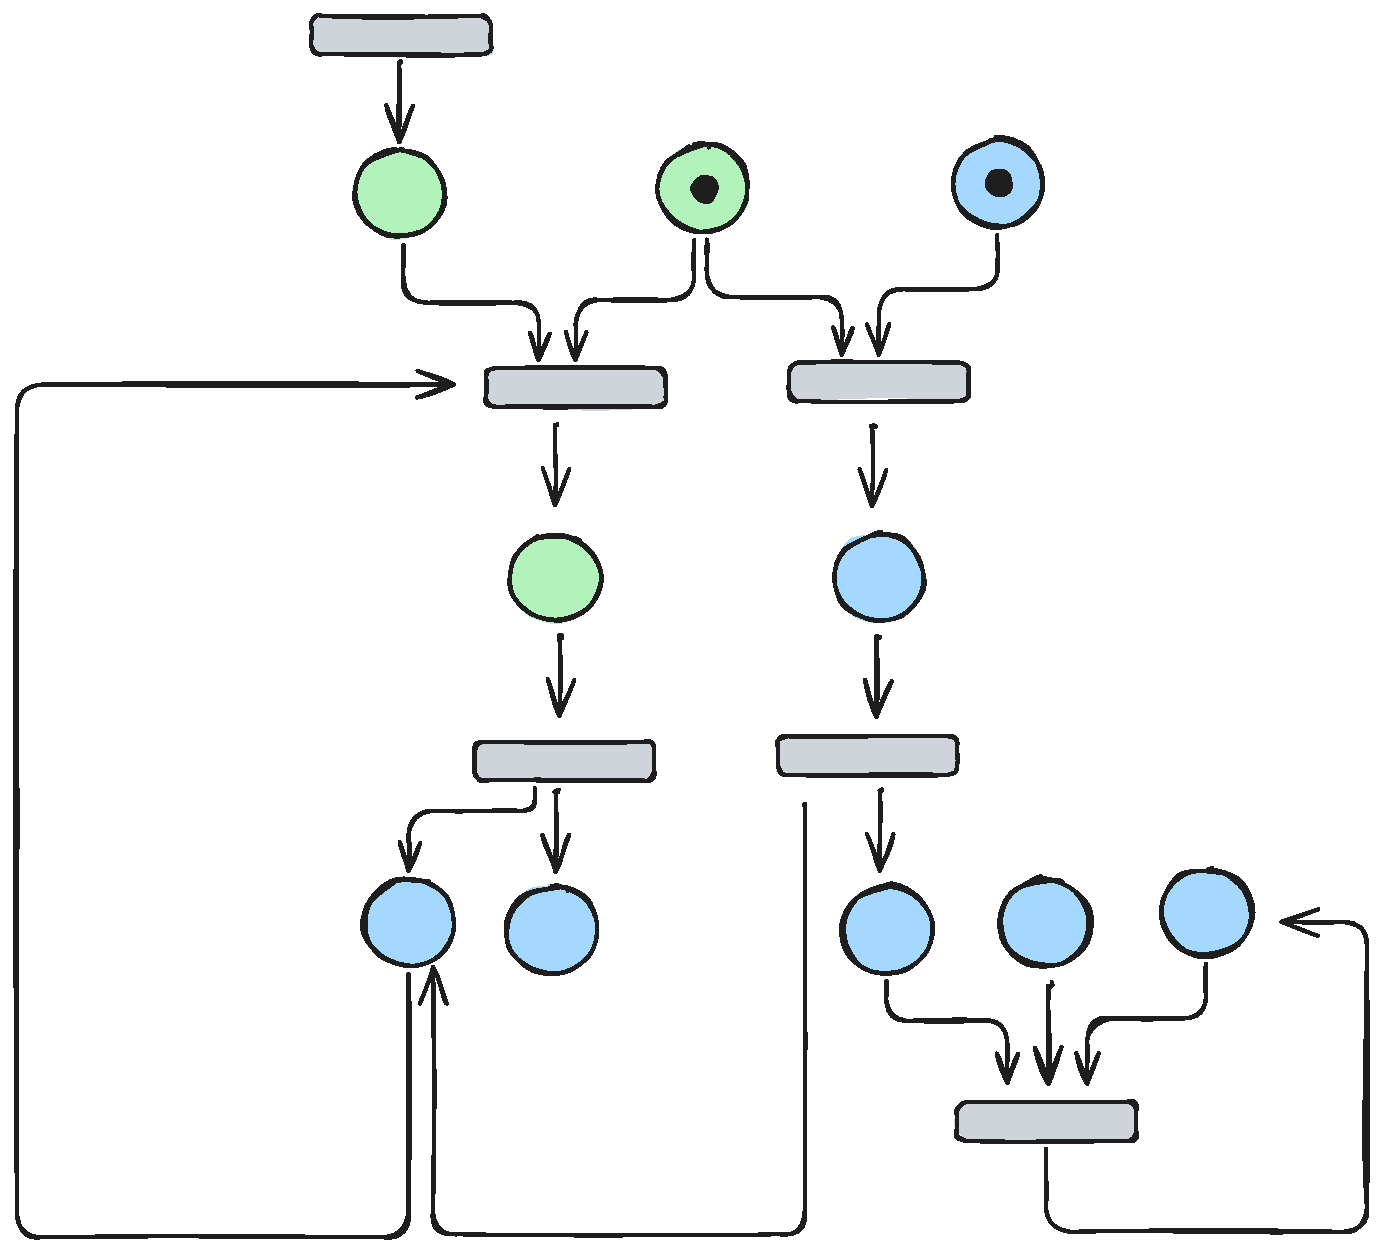
\includegraphics[width=\textwidth]{plots/bidirectional_pruning_step_a_updated.pdf}
		\caption{Step 0: initial Petri Net, before pruning.}
		\label{fig:step:a}
	\end{subfigure}\hfill
	\begin{subfigure}[b]{0.45\textwidth}
		\centering
		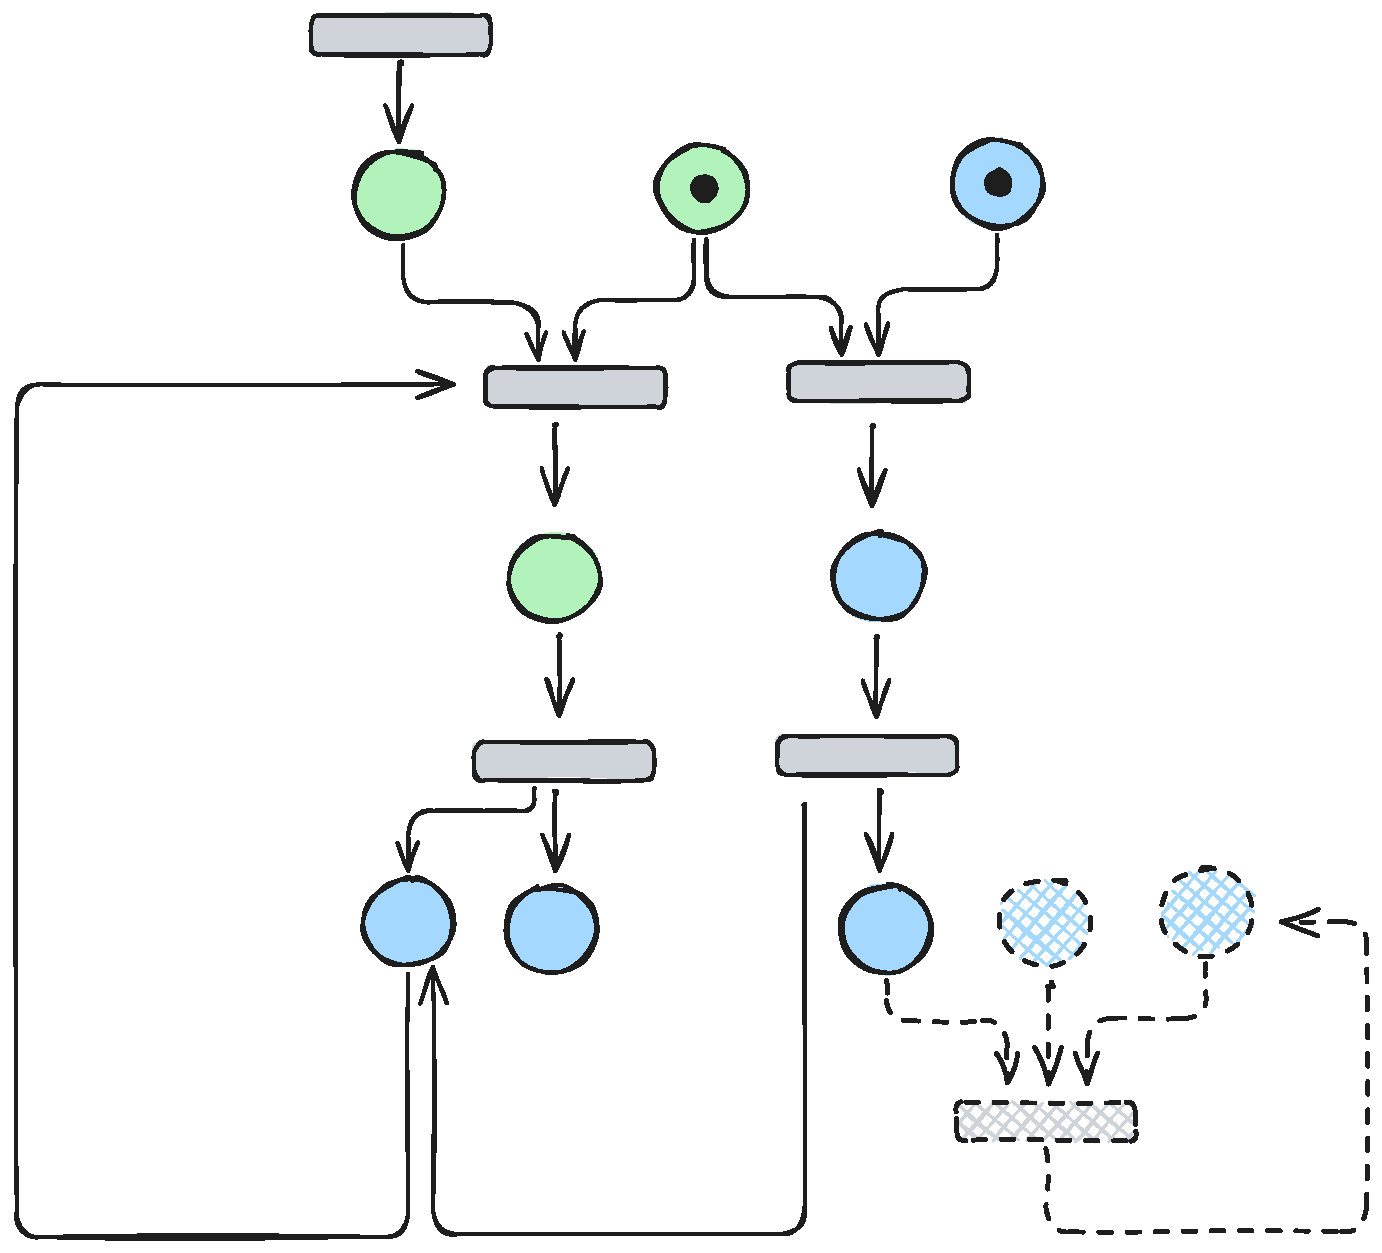
\includegraphics[width=\textwidth]{plots/bidirectional_pruning_step_b_updated.pdf}
		\caption{Step 1: first forward pass.}
		\label{fig:step:b}
	\end{subfigure}
	
	\vspace{1em}
	
	% Bottom row: (c), (d), and (e) matching (d)’s height
	\begin{subfigure}[b]{0.30\textwidth}
		\centering
		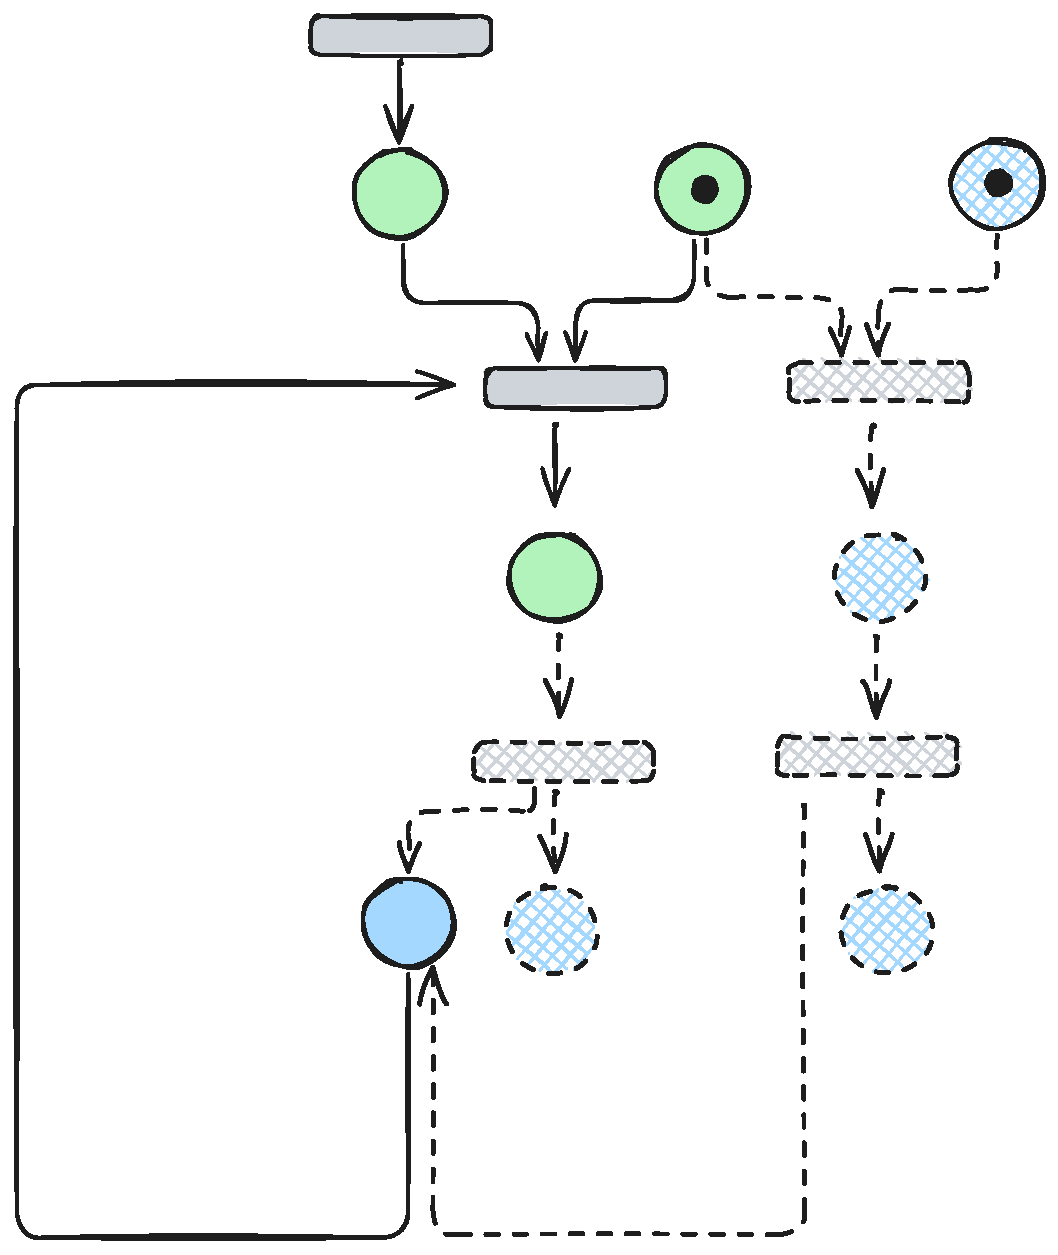
\includegraphics[width=\textwidth]{plots/bidirectional_pruning_step_c_updated.pdf}
		\caption{Step 3: first backward pass.}
		\label{fig:step:c}
	\end{subfigure}\hfill
	\begin{subfigure}[b]{0.23\textwidth}
		\centering
		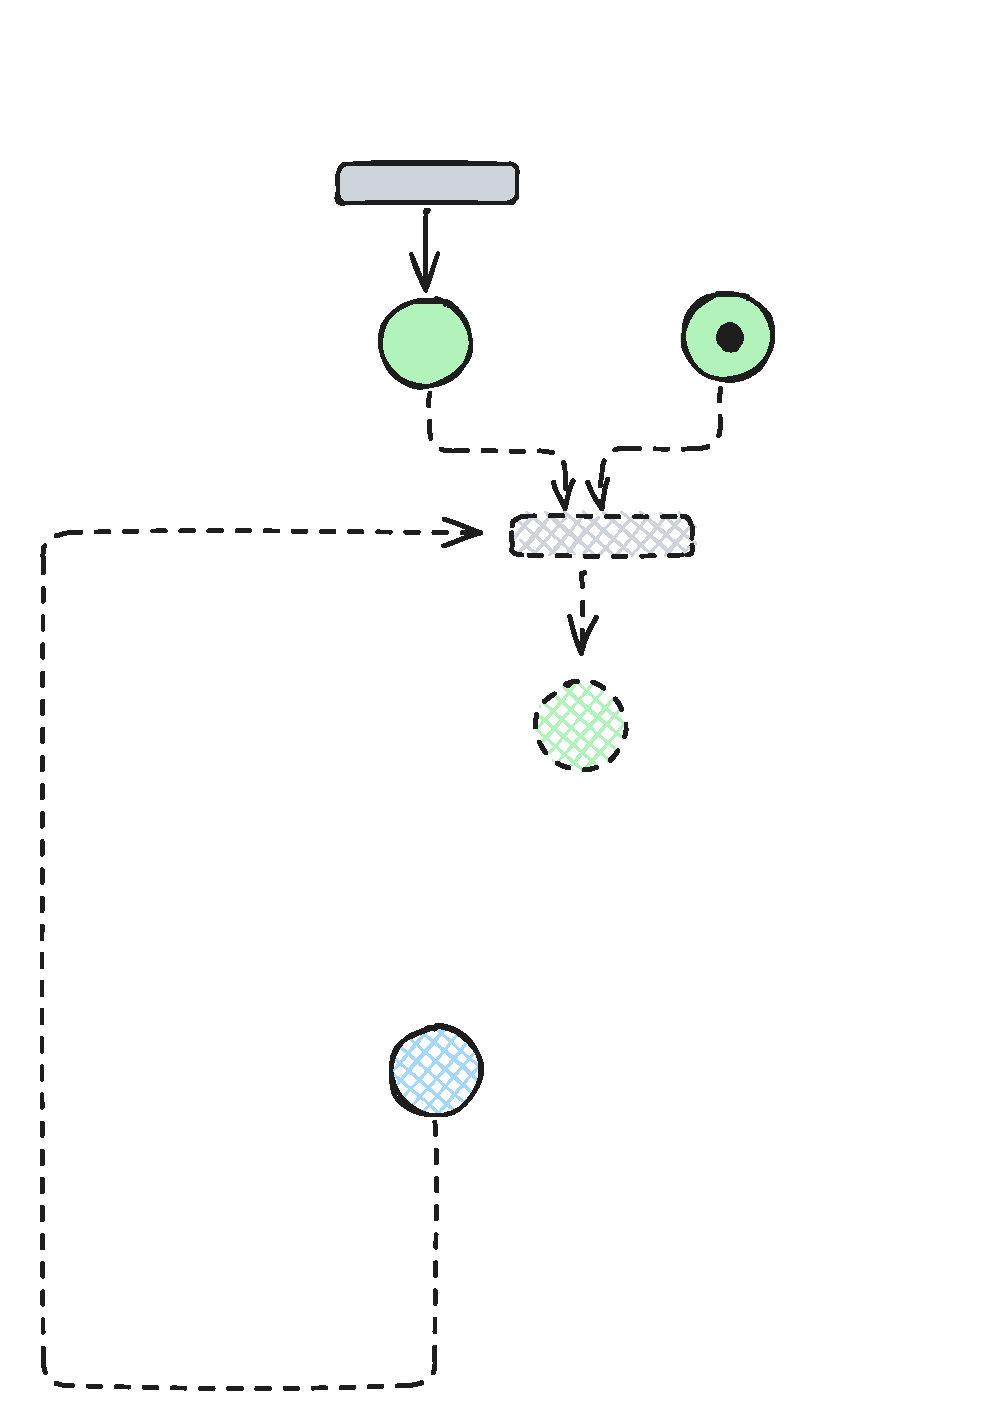
\includegraphics[width=\textwidth]{plots/bidirectional_pruning_step_d_updated_2.pdf}
		\caption{Step 4: second forward pass.}
		\label{fig:step:d}
	\end{subfigure}\hfill
	% <-- three-arg form: [vpos][total height][inner vpos]
	\begin{subfigure}[b][\subfigheight][b]{0.23\textwidth}
		\centering
		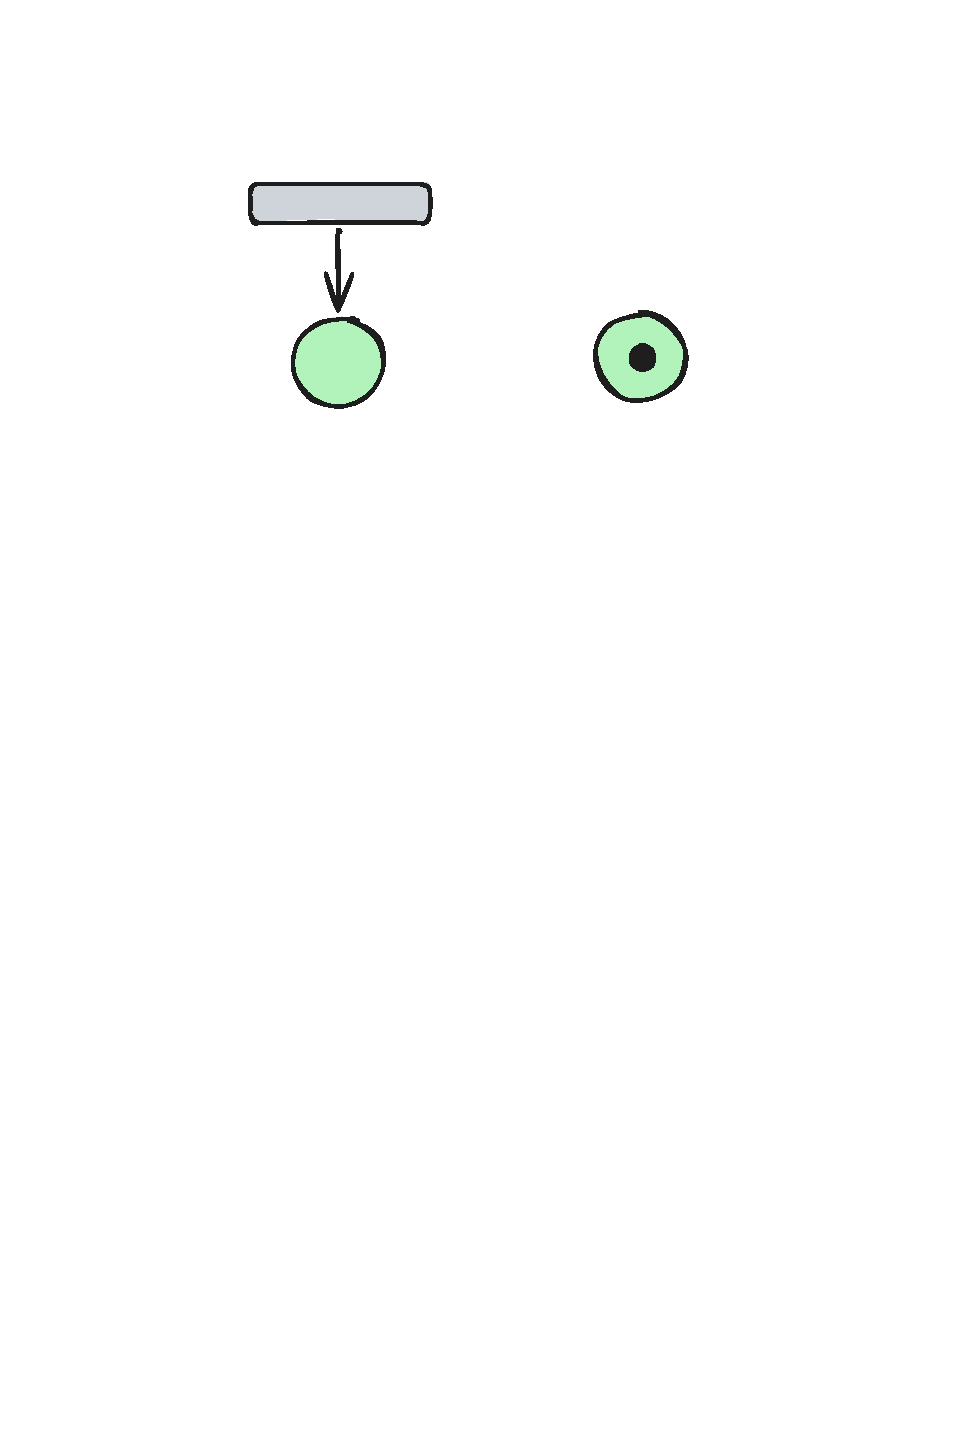
\includegraphics[width=\textwidth]{plots/bidirectional_pruning_step_e_updated_2.pdf}
		\caption{Step 6: final Petri Net.}
		\label{fig:step:e}
	\end{subfigure}
	
	\caption{A Petri net after three rounds of bidirectional pruning: two forward passes and one backward pass. Black dots represent initial token markings; green places represent places that are allowed to be reachable in our constraints (i.e., aren't fixed to zero tokens in the final marking). Dashed shapes represent places and transitions that are identified as removable in the current iteration, and will be removed after it ends.}
	\label{fig:bidirectional_pruning}
\end{figure}

%\newpage
